\subsubsection{Actuator-count ablation}
\label{subsec:multi_input_comparison}

To quantify the performance cost of restricting actuation to one node, nominal PPO synchronization is evaluated for every nonempty subset of the three nodes: $\{1\}$, $\{2\}$, $\{3\}$, $\{1,2\}$, $\{1,3\}$, $\{2,3\}$, and $\{1,2,3\}$. For a subset $\mathcal S$, the input matrix contains the corresponding columns of $I_3$, and the policy produces $|\mathcal S|$ actions. The six-dimensional observation, error-only reward, initial-state distribution, RK4 integration, policy hidden layers, PPO hyperparameters, and nominal training budget of $4\times10^5$ transitions are unchanged. Each configuration includes three independent training runs and is evaluated on 20 common test initial conditions. All seven configurations and all three final checkpoints per configuration are reported, including configurations with poor synchronization.

The same per-actuator bound $|u_j|\leq4$ is imposed in every configuration, while $E_u$ sums energy across all active channels. Thus, additional actuators provide both additional control directions and a larger admissible total input magnitude ($\|\mathbf u\|_2\leq4\sqrt{|\mathcal S|}$). This is an actuator-availability comparison, not a comparison at fixed aggregate control authority. Only nominal synchronization is tested in this ablation. Actuator count measures the structural actuation requirement; hardware cost and implementation overhead are not measured.

\begin{table}[pos=htbp,width=\linewidth]
\centering\small
\setlength{\tabcolsep}{4pt}
\caption{Nominal PPO ablation over all nonempty actuator subsets. Each configuration uses three final policies and 20 common test initial conditions per policy. Values are mean $\pm$ SD across training-seed means; energy is summed over all active inputs.}
\label{tab:multi_input_comparison}
\begin{tabular}{@{}ccccc@{}}
\toprule
Controlled nodes & Inputs & MAE & Steady L1 error & $E_u$ \\
\midrule
$\{1\}$ & 1 & $1.3937 \pm 0.0029$ & $4.2825 \pm 0.1571$ & $266.49 \pm 13.41$ \\
$\{2\}$ & 1 & $0.0930 \pm 0.0022$ & $0.0426 \pm 0.0131$ & $9.09 \pm 1.53$ \\
$\{3\}$ & 1 & $0.0431 \pm 0.0012$ & $0.0091 \pm 0.0033$ & $6.54 \pm 0.34$ \\
$\{1,2\}$ & 2 & $0.1145 \pm 0.0110$ & $0.0679 \pm 0.0212$ & $20.61 \pm 1.28$ \\
$\{1,3\}$ & 2 & $0.0232 \pm 0.0007$ & $0.0119 \pm 0.0019$ & $10.93 \pm 0.12$ \\
$\{2,3\}$ & 2 & $0.0205 \pm 0.0011$ & $0.0141 \pm 0.0040$ & $8.15 \pm 0.27$ \\
$\{1,2,3\}$ & 3 & $0.0118 \pm 0.0007$ & $0.0105 \pm 0.0026$ & $10.91 \pm 0.17$ \\
\bottomrule
\end{tabular}
\end{table}


\begin{figure}[pos=htbp,width=\linewidth]
  \centering
  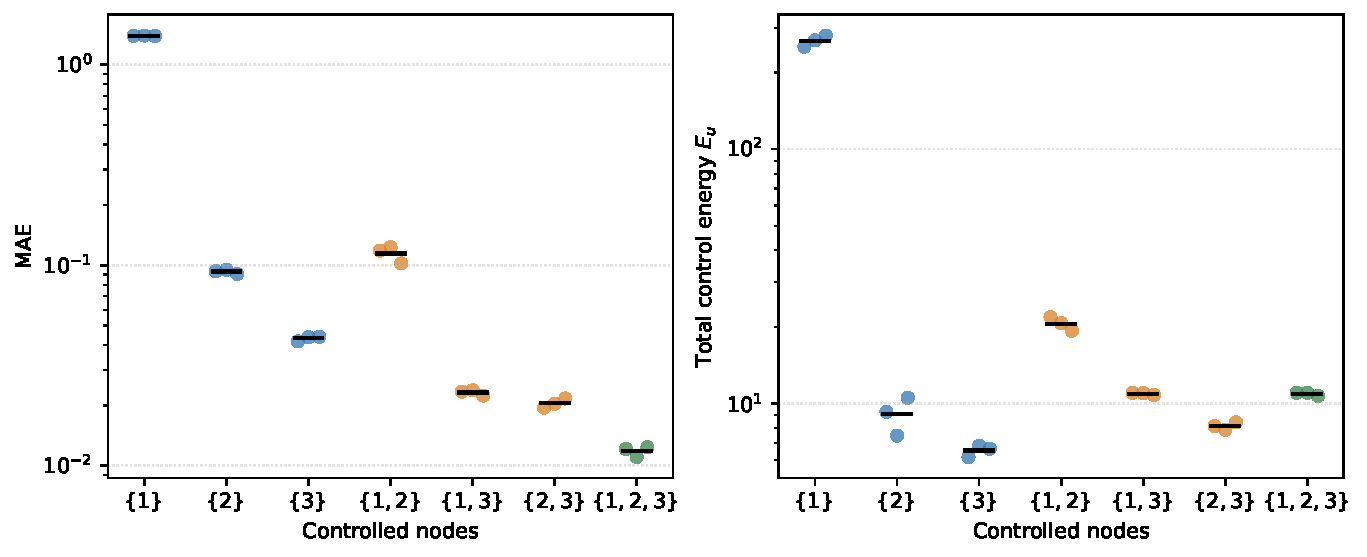
\includegraphics[width=0.96\linewidth]{figures/multi_input_matched_budget.pdf}
  \caption{Nominal synchronization error and total control energy for all actuator subsets. Each colored point is a training-seed mean over 20 common test initial conditions; black horizontal marks denote the mean across three seeds. Blue, orange, and green indicate one, two, and three actuators, respectively.}
  \label{fig:multi_input_comparison}
\end{figure}

Table~\ref{tab:multi_input_comparison} and Fig.~\ref{fig:multi_input_comparison} quantify the tradeoff. Single-node control at Node 3 gives MAE 0.0431 and energy 6.54, whereas $\{2,3\}$ gives 0.0205 and 8.15 and $\{1,2,3\}$ gives 0.0118 and 10.91. Thus, one actuator retains low-residual synchronization with lower measured energy, but incurs a higher full-horizon error than these multi-input configurations. The steady L1 error does not decrease monotonically with actuator count: it is 0.0091 for $\{3\}$, compared with 0.0141 for $\{2,3\}$ and 0.0105 for $\{1,2,3\}$. The full-horizon improvement should therefore not be described as uniformly better steady-state precision.

The $\{1,2\}$ configuration has higher MAE and energy than $\{2\}$ under the fixed training budget, while configurations containing Node 3 perform better in full-horizon MAE. This emphasizes the effect of actuator placement and finite-budget policy optimization. Since adding an actuator enlarges the admissible control set, the poorer learned result for $\{1,2\}$ is not evidence that the extra actuator intrinsically reduces controllability. These results support single-input control as a resource-constrained design choice, with an explicit performance cost, rather than as the best-performing architecture for every objective.
